%=========================================================
\chapter{Modelo dinámico}	
\label{cap:modDinamico}

	Este capítulo describe en modelo dinámico del sistema. en el se detallan todos los escenarios de ejecución del sistema. La figura~\ref{fig:casosDeUso} muestra el diagrama general del sistema y sus sib sistemas, y la figura~\ref{fig:casosDeUsoDetalle} muestra todos los casos de uso del sistema. En este documento solo detallamos los casos de uso del subsistema de gestión de cursos.
	
\begin{figure}[htbp]
	\begin{center}
		\fbox{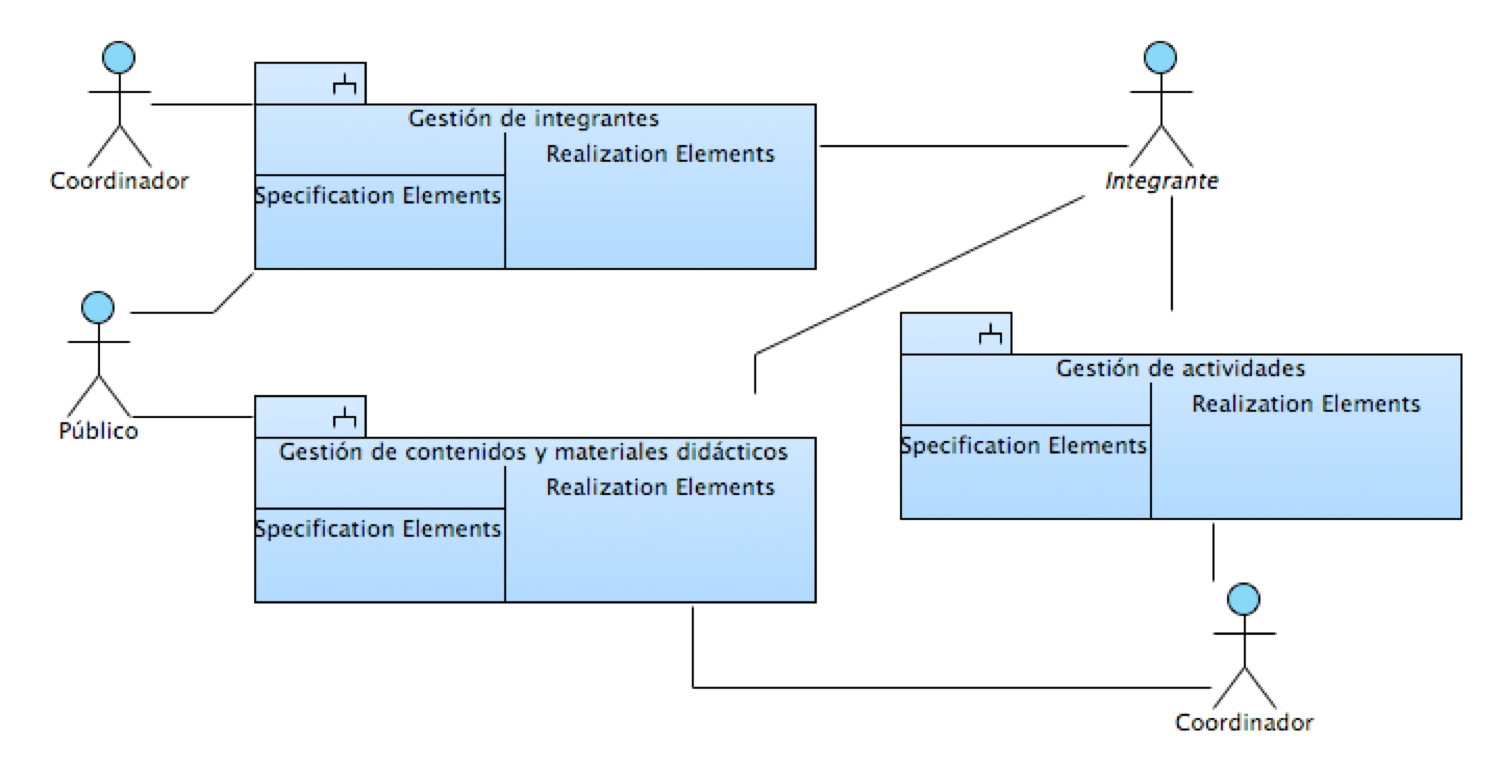
\includegraphics[width=.8\textwidth]{images/casosDeUso}}
		\caption{Diagrama de casos de uso del sistema.}
		\label{fig:casosDeUso}
	\end{center}
\end{figure}

\begin{figure}[htbp]
	\begin{center}
		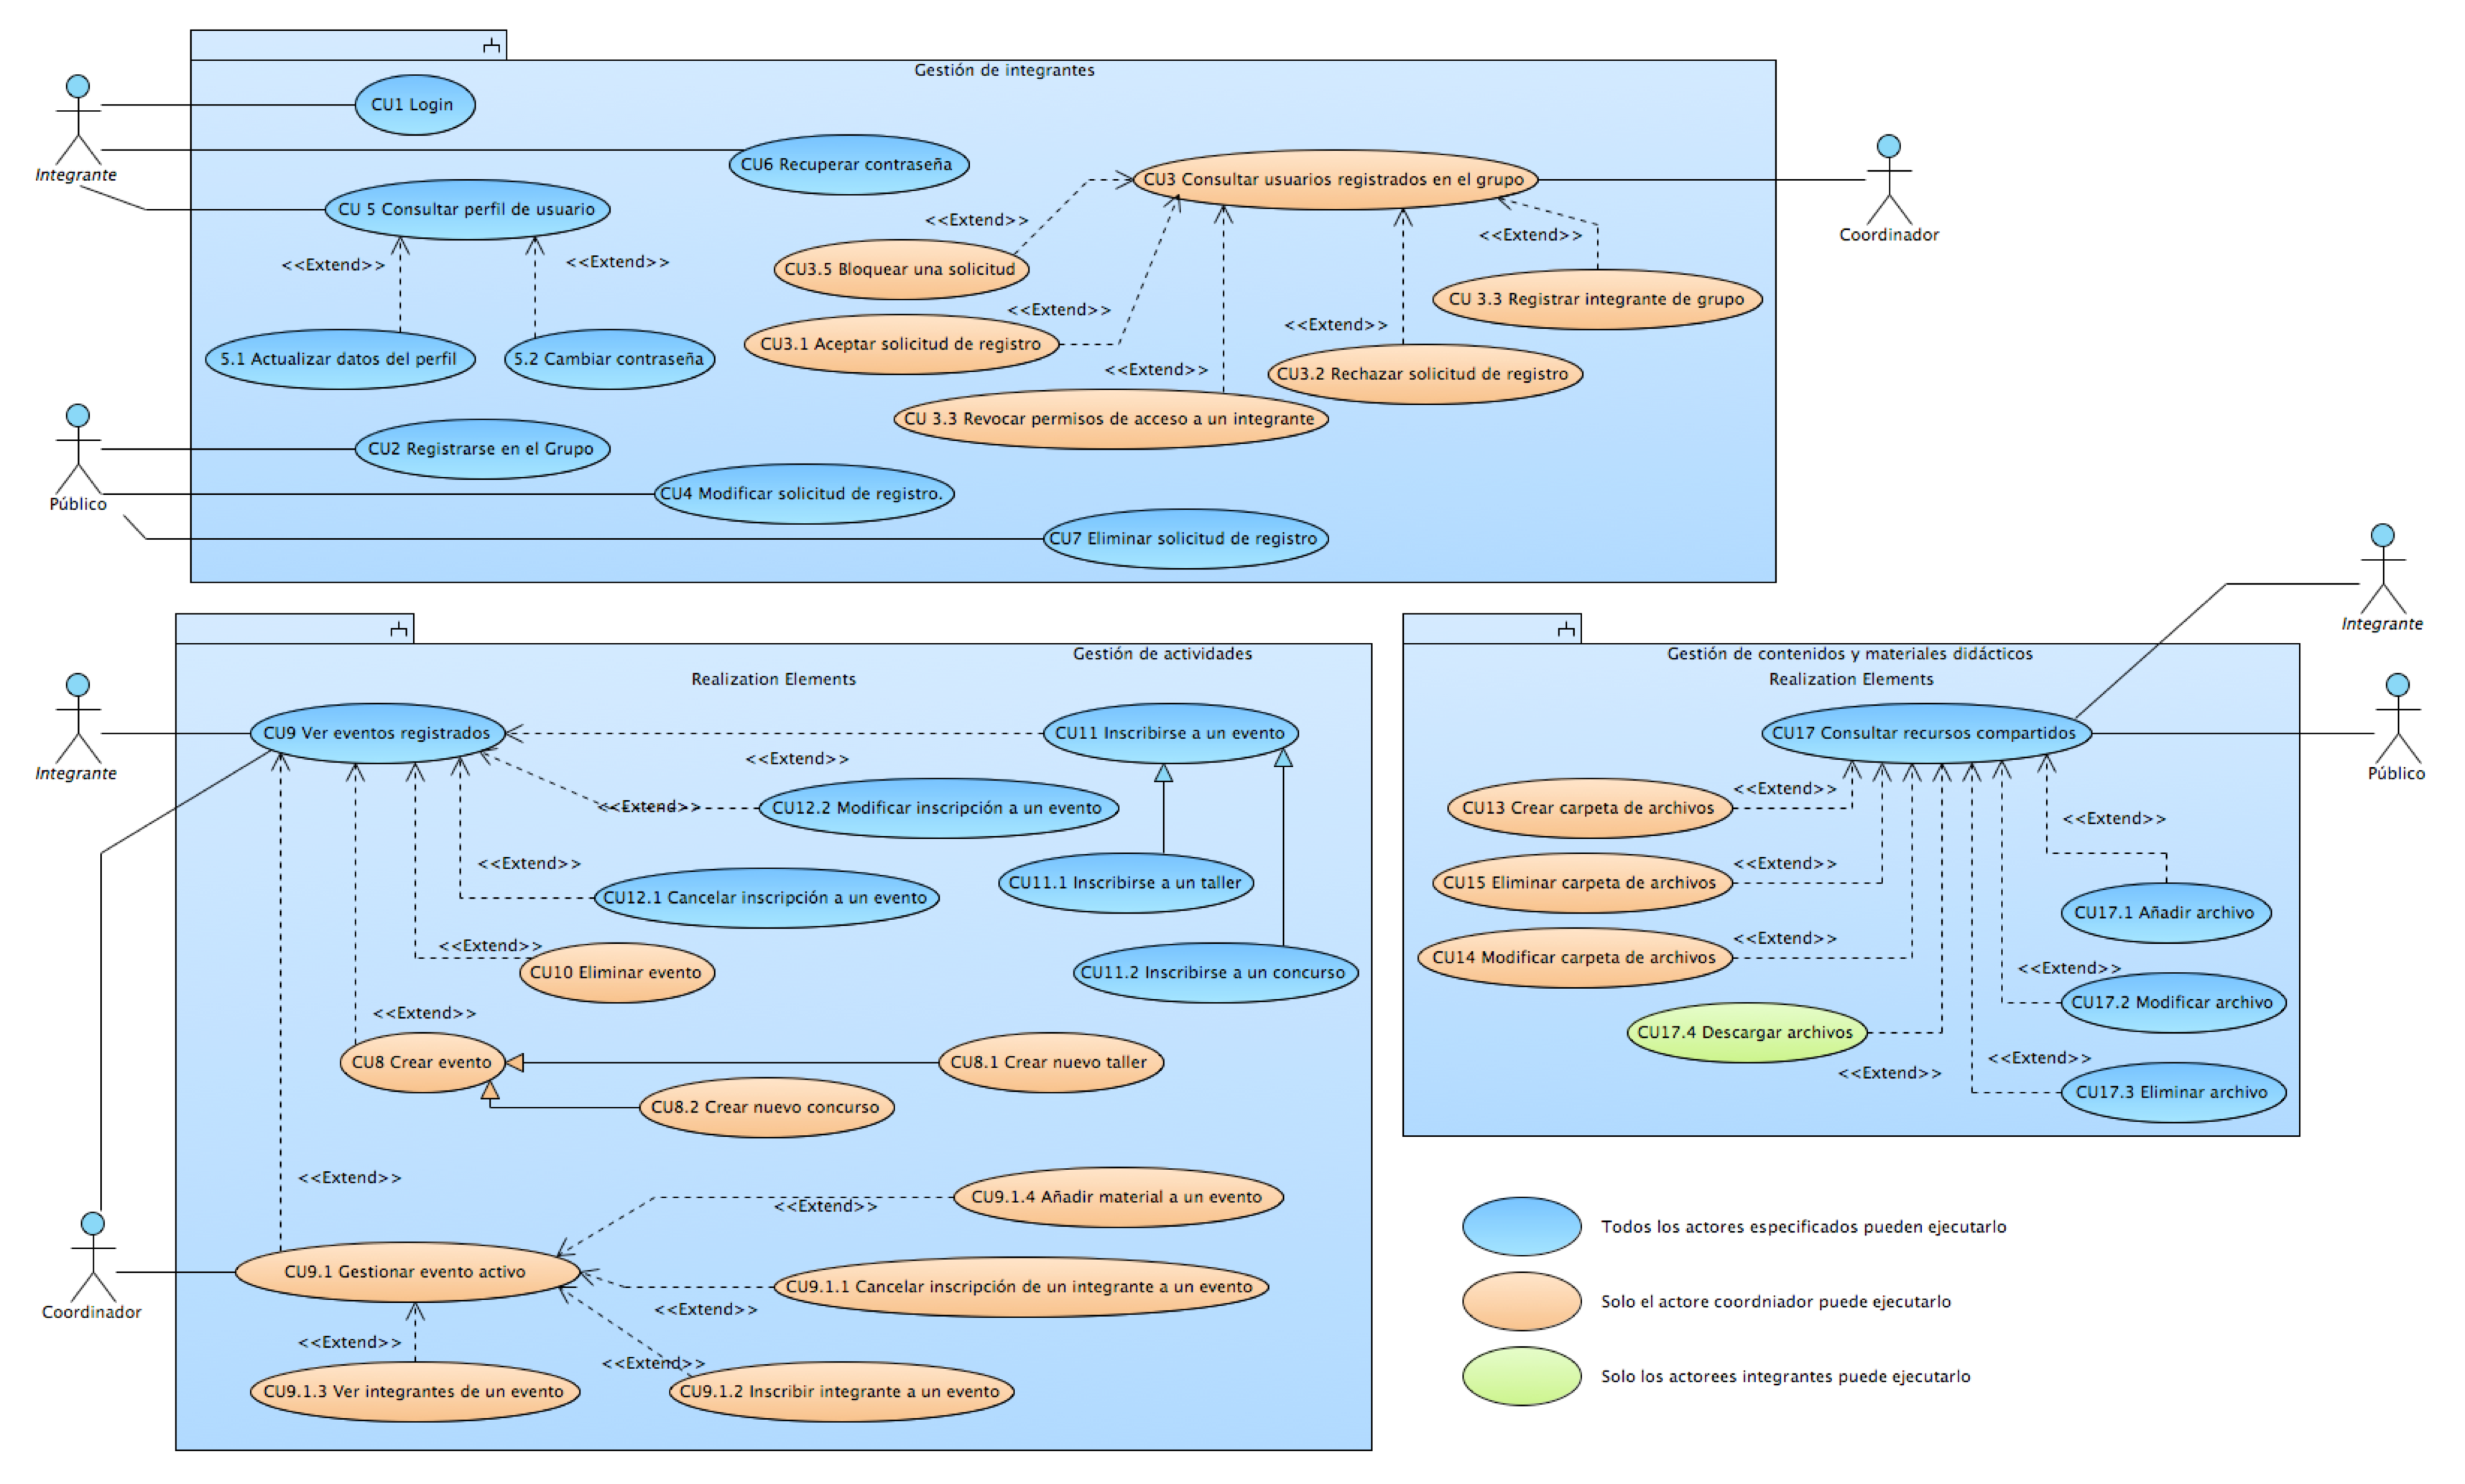
\includegraphics[angle=90, width=.7\textwidth]{images/casosDeUsoDetalle}
		\caption{Diagrama detallado del sistema.}
		\label{fig:casosDeUsoDetalle}
	\end{center}
\end{figure}

%---------------------------------------------------------
\section{Descripción de actores}

%---------------------------------------------------------
\begin{Usuario}{\hypertarget{getenteOperaciones}{\subsection{Gerente de Operaciones}}}{
	Es el encargado de todas las operaciones de la empresa y está por encima de los ejecutivos de producción y de ventas principalmente.
}
    \item[Responsabilidades:] \cdtEmpty
    \begin{itemize}
		\item Supervisar la operación.
		\item Plantear y supervisar el logro de las metas de la empresa y su crecimiento económico.
		\item ...
    \end{itemize}

	\item[Perfil:] \cdtEmpty
    \begin{itemize}
		\item Amplia experiencia en el ramo.
		\item Licenciatura como mínimo.
		\item ...
    \end{itemize}
\end{Usuario}

A continuación se detallan los casos de uso.

%---------------------------------------------------------
% CASOS DE USO

% \IUref{IUAdmPS}{Administrar Planta de Selección}
% \IUref{IUModPS}{Modificar Planta de Selección}
% \IUref{IUEliPS}{Eliminar Planta de Selección}

% 


% Copie este bloque por cada caso de uso:
%-------------------------------------- COMIENZA descripción del caso de uso.

%\begin{UseCase}[archivo de imágen]{UCX}{Nombre del Caso de uso}{
%--------------------------------------
	\begin{UseCase}{CU17}{Inscribir a Seminario}{
		Ayudar a que los Estudiantes que están por terminar la carrera se puedan inscribir en un Seminario de titulación.
	}
		\UCitem{Versión}{\color{Gray}0.1}
		\UCitem{Autor}{\color{Gray}David Ortega Pacheco}
		\UCitem{Supervisa}{\color{Gray}Ulises Vélez Saldaña.}
		\UCitem{Actor}{\hyperlink{Alumno}{Alumno}}
		\UCitem{Propósito}{Que el Estudiante se pueda inscribir a un seminario de titulación.}
		\UCitem{Entradas}{Número de boleta, Contraseña y Seminario.}
		\UCitem{Origen}{Teclado}
		\UCitem{Salidas}{Seminarios registrados, horario actual del Estudiante, desglose del monto a pagar por la inscripción, recibo de pago y comprobante de inscripción.}
		\UCitem{Destino}{Pantalla e impresora para recibo de pago y comprobante de inscripción}
		\UCitem{Precondiciones}{El estudiante debe estar registrado en la universidad.}
		\UCitem{Postcondiciones}{El estudiante quedará inscrito en el Seminario seleccionado si es elegible y hay cupo en el Seminario en cuestión.}
		\UCitem{Errores}{}
		\UCitem{Tipo}{Caso de uso primario}
		\UCitem{Observaciones}{}
	\end{UseCase}
%--------------------------------------
	\begin{UCtrayectoria}{Principal}
		\UCpaso[\UCactor] Introduce su Número de Boleta y Contraseña en el sistema vía la  \IUref{IU23}{Pantalla de Control de Acceso}\label{CU17Login}.
		\UCpaso[\UCactor] Confirma la operación presionando el botón \IUbutton{Entrar}.
		\UCpaso Verifica que el Estudiante sea elegible para inscribirse al Seminario con base en la regla \BRref{BR129}{Determinar si un Estudiante puede inscribir Seminario.} \Trayref{A}.
		\UCpaso Despliega la \IUref{IU32}{Pantalla de Selección de Seminario} con la lista de Seminarios Disponibles.
		\UCpaso[\UCactor] Selecciona el Seminario en el que desea inscribirse \Trayref{B}\label{CU17SeleccionarSeminario}.
		\UCpaso Verifica que el Estudiante sea elegible para inscribirse al seminario seleccionado con base en la regla \BRref{BR130}{Determinar si un Estudiante puede inscribirse en un Seminario} \Trayref{C}.
		\UCpaso Verifica que el horario del Seminario concuerde con el horario del Estudiante con base en la regla \BRref{BR143}{Validar el horario del estudiante} \Trayref{D}.
		\UCpaso Calcula el costo del Seminario basado en el costo publicado en el catálogo de cursos, los costos aplicables al alumno y los impuestos aplicables, con base en las reglas \BRref{BR180}{Calcular costos del Estudiante} y \BRref{BR45}{Calcular impuestos por seminario}.
		\UCpaso Despliega el desglose de costos en la \IUref{IU33}{Pantalla Mostrar costos por seminario}.
		\UCpaso Pide al Estudiante que confirme la inscripción alSeminario.
		\UCpaso[\UCactor] Confirma la inscripción al Seminario.
		\UCpaso Inscribe al Estudiante en el Seminario seleccionado.
		\UCpaso Informa que la inscripción se realizó exitosamente vía la \IUref{UI88}{Pantalla de resumen de inscripción al Seminario}. 
		\UCpaso Imprime el recibo de pago con base en la regla \BRref{BR100}{Recibo del Estudiante por inscripción a Seminario.}.
		\UCpaso Pregunta al estudiante si desea imprimir un comprobante de la inscripción.
		\UCpaso[\UCactor] Indica que desea imprimir el comprobante de la inscripción.
		\UCpaso Imprime el comprobante de la inscripción \IUref{IU189}{Reporte de inscripción a Seminario}.		
	\end{UCtrayectoria}

%--------------------------------------		
		\begin{UCtrayectoriaA}{A}{El Estudiante no puede inscribir un Seminario}
			\UCpaso Muestra el Mensaje {\bf MSG1-}``El Estudiante [{\em Número de Boleta}] aun no puede inscribirse al seminario.''.
			\UCpaso[\UCactor] Oprime el botón \IUbutton{Aceptar}.
			\UCpaso[] Termina el caso de uso.
		\end{UCtrayectoriaA}
		
%--------------------------------------
		\begin{UCtrayectoriaA}{B}{El Estudiante abandona la operación}
			\UCpaso El Estudiante revisa la lista de Seminarios y no encuentra el Seminario que desea.
			\UCpaso[\UCactor] Oprime el botón \IUbutton{Salir}.
			\UCpaso Cierra la sesión del usuario.
			\UCpaso Continua en el paso \ref{CU17Login} del \UCref{CU17}.
		\end{UCtrayectoriaA}

%--------------------------------------
		\begin{UCtrayectoriaA}{C}{El estudiante no cumple con los prerrequicitos}
			\UCpaso Muestra el Mensaje {\bf MSG2-}``El Estudiante [{\em Número de Boleta}] no cumple con los requisitos para inscribirse al Seminario [{\em Nombre del Seminario seleccionado}].''.
			\UCpaso Muestra los requisitos que el Seminario seleccionado solicita.
			\UCpaso Continúa en el paso \ref{CU17SeleccionarSeminario} del \UCref{CU17}.
		\end{UCtrayectoriaA}

%--------------------------------------
		\begin{UCtrayectoriaA}{D}{El horario es incompatible.}
			\UCpaso Muestra el Mensaje {\bf MSG3-}``El horario del [{\em Nombre del Seminario seleccionado}] no es compatible con el horario del curso [{\em Nombre de la materia y grupo del curso con el que choca el horario}].''.
			\UCpaso Continúa en el paso \ref{CU17SeleccionarSeminario} del \UCref{CU17}.
		\end{UCtrayectoriaA}

%--------------------------------------
% Puntos de extensión
\subsection{Puntos de extensión}
\UCExtenssionPoint{
	% Cuando:
	Desea conocer las materias cursadas.
}{
	% Durante la región:
	Del paso 4 al paso 9.
}{
	% Casos de uso a los que extiende:
	\hyperlink{CU3.4}{CU3.4 Consultar historial académico}.
}
		
		
		
%-------------------------------------- TERMINA descripción del caso de uso.



